% \documentclass[svgnames]{article}
% To make png: pdftopng -r 900 -alpha LucasBoston.pdf temp.png
\documentclass[svgnames,convert={density=900,size=1400x1200,outext=.png}]{standalone}
\usepackage{tikz}
\usetikzlibrary{calc,trees,positioning,arrows,chains,shapes.geometric,backgrounds,
  decorations.pathreplacing,decorations.pathmorphing,shapes,snakes,automata,
  matrix,shapes.symbols,mindmap,shadows,petri}
% \renewcommand{\rmdefault}{phv} % Arial
% \renewcommand{\sfdefault}{phv} % Arial
% \usepackage{amsmath} % to allow Sans font in math


\begin{document}
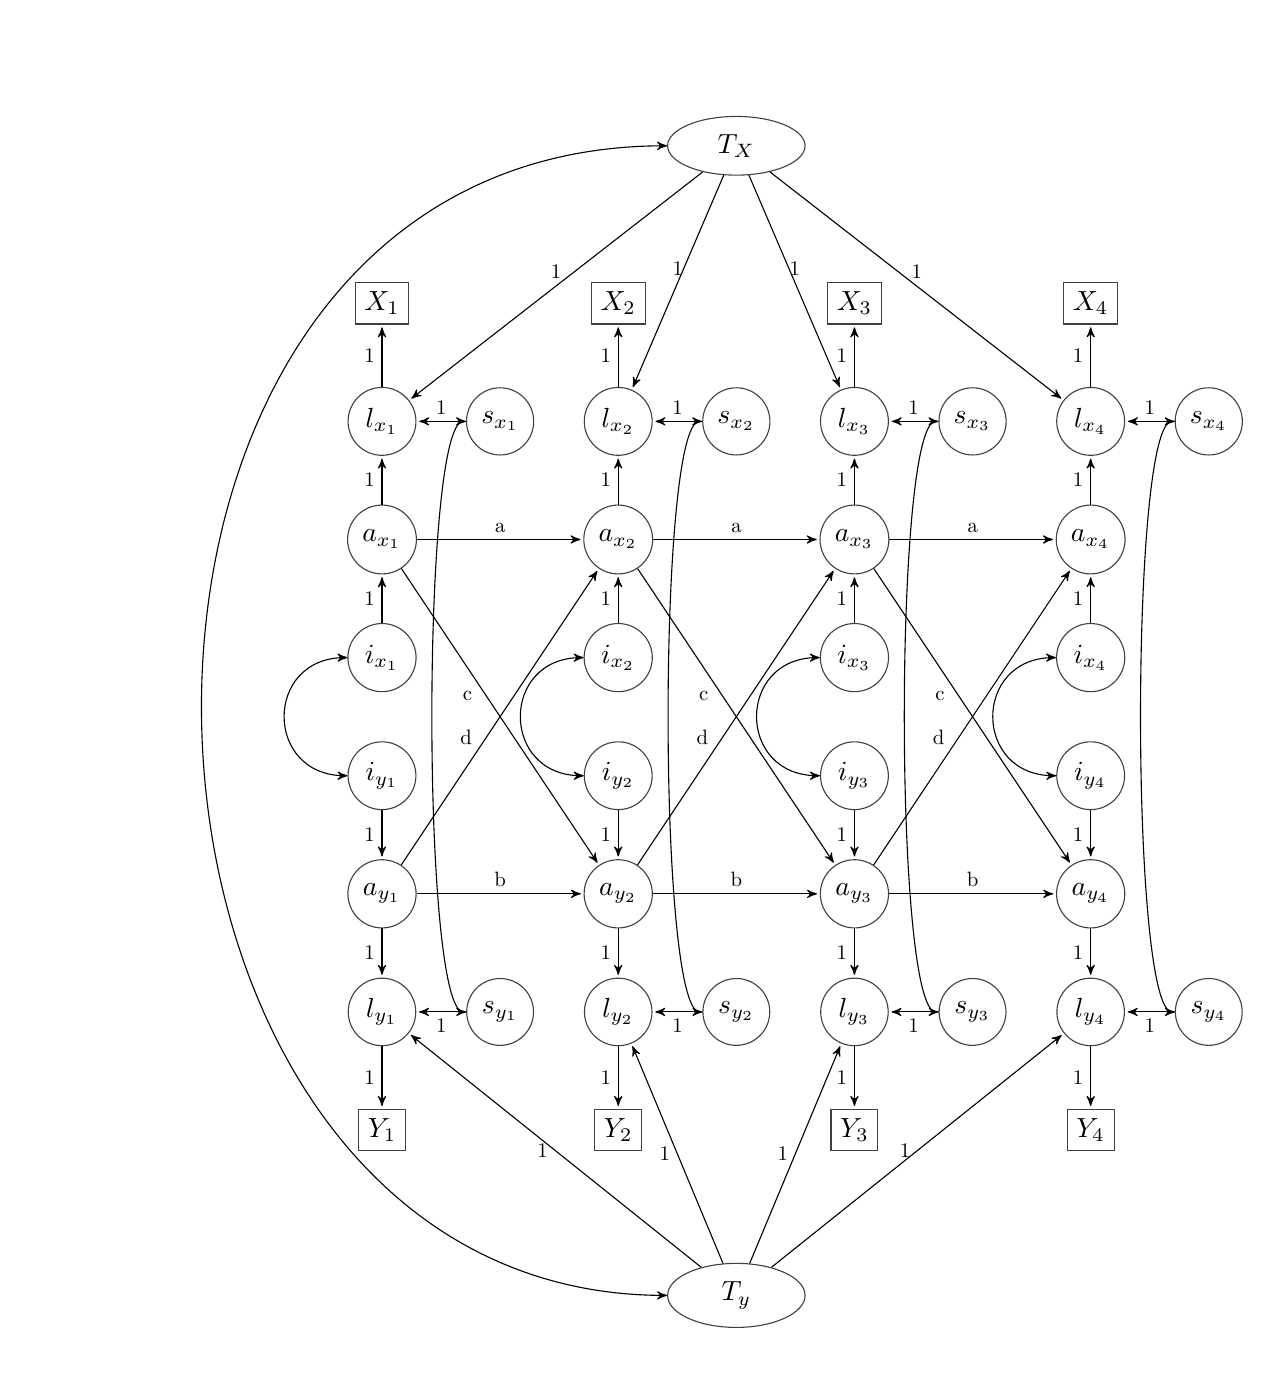
\begin{tikzpicture}[node distance=1.8cm,>=stealth',bend angle=45,auto]
  \useasboundingbox (-9,-15) rectangle (6.5,2);
%%  \useasboundingbox (-7.5,-3) rectangle (5.5,7);
  \tikzset{
    latentTrait/.style={ellipse,draw=black!75,minimum size=3mm, text width=10mm, align=center},
    latentAR/.style={ellipse,draw=black!75,minimum size=7mm},
    component/.style={circle,draw=black!75,minimum size=7mm, align=center},
    observed/.style={rectangle,draw=black!75,minimum size=5mm, align=center},
    error/.style={circle,draw=black!75,minimum size=.9mm},
    errorAR/.style={circle,draw=black!75,minimum size=1mm, node distance=.73cm},
    state/.style={circle,draw=black!75,minimum size=1mm, scale=.75, align=center, node distance=1.7cm},
    hspace/.style={node distance=2.7cm},
    vspace/.style={node distance=4.25cm},
    % edge styles
    standardDist/.style={node distance=1.5cm},
    waveDist/.style={node distance=3cm},
    indicatorDist/.style={node distance=1.2cm},
    errorDist/.style={node distance=.73cm},
    newARDist/.style={node distance=1.2cm},
    stabDist/.style={node distance=1cm},
    %label styles
    constraints/.style={scale=.75,above},
    constraintsb/.style={scale=.75,below},
    constraintsl/.style={scale=.75,left},
    constraintsr/.style={scale=.75,right}
  }


  % Labels
  %%% STARTS
  
  % X Vars

  \node [latentTrait] (tx) at (0,.5)                        {$T_X$};

  % Wave 1 X
  \node [observed] (x1) at (-4.5,-1.5)                        {$X_1$};

  \node [component, standardDist] (l1) [below of=x1]                                            {$l_{x_1}$}
  edge [post] node[constraintsl] {1} (x1)
  edge [pre] node[constraints] {1} (tx);

  \node [component, standardDist] (a1) [below of=l1]                                            {$a_{x_1}$}
  edge [post] node[constraintsl] {1} (l1);

  \node [component, standardDist] (i1) [below of=a1]                                            {$i_{x_1}$}
  edge [post] node[constraintsl] {1} (a1);

  \node [component, standardDist] (s1) [right of=l1] {$s_{x_1}$}
  edge [post] node[constraints] {1} (l1);

  % Wave 2 X
  \node [observed, waveDist] (x2) [right of=x1]                         {$X_2$};

  \node [component, standardDist] (l2) [below of=x2]                                            {$l_{x_2}$}
  edge [post] node[constraintsl] {1} (x2)
  edge [pre] node[constraints] {1} (tx);

  \node [component, standardDist] (a2) [below of=l2]                                            {$a_{x_2}$}
  edge [post] node[constraintsl] {1} (l2)
  edge [pre] node[constraints] {a} (a1);

  \node [component, standardDist] (i2) [below of=a2]                                            {$i_{x_2}$}
  edge [post] node[constraintsl] {1} (a2);

  \node [component, standardDist] (s2) [right of=l2] {$s_{x_2}$}
  edge [post] node[constraints] {1} (l2);

  % Wave 3 X
  \node [observed, waveDist] (x3) [right of=x2]                         {$X_3$};

  \node [component, standardDist] (l3) [below of=x3]                                            {$l_{x_3}$}
  edge [post] node[constraintsl] {1} (x3)
  edge [pre] node[constraints] {1} (tx);

  \node [component, standardDist] (a3) [below of=l3]                                            {$a_{x_3}$}
  edge [post] node[constraintsl] {1} (l3)
  edge [pre] node[constraints] {a} (a2);

  \node [component, standardDist] (i3) [below of=a3]                                            {$i_{x_3}$}
  edge [post] node[constraintsl] {1} (a3);

  \node [component, standardDist] (s3) [right of=l3] {$s_{x_3}$}
  edge [post] node[constraints] {1} (l3);

  % Wave 4 X
  \node [observed, waveDist] (x4) [right of=x3]                         {$X_4$};

  \node [component, standardDist] (l4) [below of=x4]                                            {$l_{x_4}$}
  edge [post] node[constraintsl] {1} (x4)
  edge [pre] node[constraints] {1} (tx);

  \node [component, standardDist] (a4) [below of=l4]                                            {$a_{x_4}$}
  edge [post] node[constraintsl] {1} (l4)
  edge [pre] node[constraints] {a} (a3);

  \node [component, standardDist] (i4) [below of=a4]                                            {$i_{x_4}$}
  edge [post] node[constraintsl] {1} (a4);

  \node [component, standardDist] (s4) [right of=l4] {$s_{x_4}$}
  edge [post] node[constraints] {1} (l4);




  %% Y
  \node [latentTrait, node distance=14.6cm] (ty) [below of=tx]                        {$T_y$};

  \node [component, standardDist] (iy1) [below of=i1]                                            {$i_{y_1}$};
  \node [component, standardDist] (ay1) [below of=iy1] {$a_{y_1}$}
  edge [pre] node[constraintsl] {1} (iy1)
  edge [post] node[constraintsl, yshift=-10pt, xshift=-10pt] {d} (a2);

  \node [component, standardDist] (ly1) [below of=ay1] {$l_{y_1}$}
  edge [pre] node[constraintsl] {1} (ay1)
  edge [pre] node[constraintsl] {1} (ty);

  \node [observed, standardDist] (y1) [below of=ly1] {$Y_1$}
  edge [pre] node[constraintsl] {1} (ly1);

  \node [component, standardDist] (sy1) [right of=ly1] {$s_{y_1}$}
  edge [post] node[constraintsb] {1} (ly1);

  % Wave 2
  \node [component, standardDist] (iy2) [below of=i2]                                    {$i_{y_2}$};
  \node [component, standardDist] (ay2) [below of=iy2] {$a_{y_2}$}
  edge [pre] node[constraintsl] {1} (iy2)
  edge [pre] node[constraints] {b} (ay1)
  edge [post] node[constraintsl, yshift=-10pt, xshift=-10pt] {d} (a3)
  edge [pre] node[constraintsl, yshift=10pt,xshift=-10pt] {c} (a1);

  \node [component, standardDist] (ly2) [below of=ay2] {$l_{y_2}$}
  edge [pre] node[constraintsl] {1} (ay2)
  edge [pre] node[constraintsl] {1} (ty);

  \node [observed, standardDist] (y2) [below of=ly2] {$Y_2$}
  edge [pre] node[constraintsl] {1} (ly2);

  \node [component, standardDist] (sy2) [right of=ly2] {$s_{y_2}$}
  edge [post] node[constraintsb] {1} (ly2);

  % Wave 3
  \node [component, standardDist] (iy3) [below of=i3]                                    {$i_{y_3}$};
  \node [component, standardDist] (ay3) [below of=iy3] {$a_{y_3}$}
  edge [pre] node[constraintsl] {1} (iy3)
  edge [pre] node[constraints] {b} (ay2)
  edge [post] node[constraintsl, yshift=-10pt, xshift=-10pt] {d} (a4)
  edge [pre] node[constraintsl, yshift=10pt,xshift=-10pt] {c} (a2);

  \node [component, standardDist] (ly3) [below of=ay3] {$l_{y_3}$}
  edge [pre] node[constraintsl] {1} (ay3)
  edge [pre] node[constraintsl] {1} (ty);

  \node [observed, standardDist] (y3) [below of=ly3] {$Y_3$}
  edge [pre] node[constraintsl] {1} (ly3);

  \node [component, standardDist] (sy3) [right of=ly3] {$s_{y_3}$}
  edge [post] node[constraintsb] {1} (ly3);

  % Wave 4
  \node [component, standardDist] (iy4) [below of=i4]                                    {$i_{y_4}$};
  \node [component, standardDist] (ay4) [below of=iy4] {$a_{y_4}$}
  edge [pre] node[constraintsl] {1} (iy4)
  edge [pre] node[constraints] {b} (ay3)
  edge [pre] node[constraintsl, yshift=10pt,xshift=-10pt] {c} (a3);

  \node [component, standardDist] (ly4) [below of=ay4] {$l_{y_4}$}
  edge [pre] node[constraintsl] {1} (ay4)
  edge [pre] node[constraintsl] {1} (ty);

  \node [observed, standardDist] (y4) [below of=ly4] {$Y_4$}
  edge [pre] node[constraintsl] {1} (ly4);

  \node [component, standardDist] (sy4) [right of=ly4] {$s_{y_4}$}
  edge [post] node[constraintsb] {1} (ly4);

  % Correlations
  \draw [<->] (tx) .. controls +(left:9cm) and +
  (left:8.5cm) .. node[sloped,above] {} (ty);
  \draw [<->] (i1) .. controls + (left:1.5cm) and +
  (left:1.5cm) .. (iy1);
  \draw [<->] (i2) .. controls + (left:1.5cm) and +
  (left:1.5cm) .. (iy2);
  \draw [<->] (i3) .. controls + (left:1.5cm) and +
  (left:1.5cm) .. (iy3);
  \draw [<->] (i4) .. controls + (left:1.5cm) and +
  (left:1.5cm) .. (iy4);
  \draw [<->] (sy1) .. controls + (left:1cm) and +
  (left:1cm) .. (s1);
  \draw [<->] (sy2) .. controls + (left:1cm) and +
  (left:1cm) .. (s2);
  \draw [<->] (sy3) .. controls + (left:1cm) and +
  (left:1cm) .. (s3);
  \draw [<->] (sy4) .. controls + (left:1cm) and +
  (left:1cm) .. (s4);



  
\end{tikzpicture}
\end{document}
